%%%%%%%%%%%%%%%%%%%%%%%%%%%%%%%%%%%%%%%%%
% Masters/Doctoral Thesis 
% LaTeX Template
% Version 1.43 (17/5/14)
%
% This template has been downloaded from:
% http://www.LaTeXTemplates.com
%
% Original authors:
% Steven Gunn 
% http://users.ecs.soton.ac.uk/srg/softwaretools/document/templates/
% and
% Sunil Patel
% http://www.sunilpatel.co.uk/thesis-template/
%
% License:
% CC BY-NC-SA 3.0 (http://creativecommons.org/licenses/by-nc-sa/3.0/)
%
% Note:
% Make sure to edit document variables in the Thesis.cls file
%
%%%%%%%%%%%%%%%%%%%%%%%%%%%%%%%%%%%%%%%%%

%----------------------------------------------------------------------------------------
%	PACKAGES AND OTHER DOCUMENT CONFIGURATIONS
%----------------------------------------------------------------------------------------

\documentclass[11pt, oneside]{Thesis} % The default font size and one-sided printing (no margin offsets)
\usepackage[francais,french]{babel}
\graphicspath{{Pictures/}} % Specifies the directory where pictures are stored
\usepackage[square, numbers, comma, sort&compress]{natbib} % Use the natbib reference package - read up on this to edit the reference style; if you want text (e.g. Smith et al., 2012) for the in-text references (instead of numbers), remove 'numbers' 
\usepackage[nottoc]{tocbibind}
\usepackage{array}
\usepackage{textcomp}
\hypersetup{urlcolor=blue, colorlinks=true} % Colors hyperlinks in blue - change to black if annoying
\usepackage{listings, xcolor}
\lstset{
	language = php,
	basicstyle = \small\ttfamily,
	keywordstyle = \color{blue},
	stringstyle = \color{red},
	identifierstyle = \color{black},
	commentstyle = \color{gray},
	emph = [1]{php},
	emphstyle = [1]\color{black},
	emph = [2]{if,and,or,else},
	emphstyle = [2]\color{dkyellow}
}
\title{\ttitle} % Defines the thesis title - don't touch this

\begin{document}

\frontmatter % Use roman page numbering style (i, ii, iii, iv...) for the pre-content pages

\setstretch{1.3} % Line spacing of 1.3

% Define the page headers using the FancyHdr package and set up for one-sided printing
\fancyhead{} % Clears all page headers and footers
\rhead{\thepage} % Sets the right side header to show the page number
\lhead{} % Clears the left side page header

\pagestyle{fancy} % Finally, use the "fancy" page style to implement the FancyHdr headers

\newcommand{\HRule}{\rule{\linewidth}{0.5mm}} % New command to make the lines in the title page
\newcolumntype{P}[1]{>{\raggedleft\arraybackslash}p{#1}}
\newcolumntype{M}[1]{>{\centering\arraybackslash}m{#1}}

\renewcommand\ttitle{Développement d'un portail de travail collaboratif}
\renewcommand\authornames{KABINE KABA}
\renewcommand\supname{M. Pascal Poizat}
\renewcommand\univname{Université Paris Ouest Nanterre La Défense}
\renewcommand\degreename{Master MIAGE}
\renewcommand\deptname{l'UFR SEGMI}
\renewcommand\acknowledgements{}
\renewcommand\abstract{Abstract}
\newcommand\resume{}
\renewcommand{\listtablename}{Liste des tableaux}
\renewcommand{\listfigurename}{Liste des figures}
\renewcommand{\FrenchLabelItem}{\textbullet}
\renewcommand{\listofsymbols}{}
\newcommand\tutornames{M. François Veyrier}





% PDF meta-data
\hypersetup{pdftitle={\ttitle}}
\hypersetup{pdfsubject=\subjectname}
\hypersetup{pdfauthor=\authornames}
\hypersetup{pdfkeywords=\keywordnames}

%----------------------------------------------------------------------------------------
%	TITLE PAGE
%----------------------------------------------------------------------------------------

\begin{titlepage}
\begin{center}

\textsc{\LARGE \univname}\\[0.5cm] % University name
%
\includegraphics[width=4.5cm]{Logo}\\[0.5cm] % University/department logo - uncomment to place it
{\includegraphics[width=4.5cm]{segmi.jpg}} \bigskip
{
\includegraphics[width=4.5cm]{erdf.jpg}}\\[.3cm]
\textsc{\Large Master II MIAGE}\\ % Thesis type
\textsc{Méthodes Informatiques Appliquées à la Gestion des Entreprise}\\[0.5cm]

\HRule \\[0.4cm] % Horizontal line
{\huge \bfseries \ttitle}\\[0.4cm] % Thesis title
\HRule \\[1.5cm] % Horizontal line
 
\begin{minipage}{0.3\textwidth}
\begin{flushleft} \large
\emph{Auteur:}\\
{\authornames} % Author name - remove the \href bracket to remove the link
\end{flushleft}
\end{minipage}
\begin{minipage}{0.3\textwidth}
\begin{center} \large
\emph{Tuteur en entreprise:}\\
{\tutornames}
\end{center}
\end{minipage}
\begin{minipage}{0.3\textwidth}
\begin{flushright} \large
\emph{Encadrant:} \\
\href{https://pages.lip6.fr/Pascal.Poizat}{\supname} % Supervisor name - remove the \href bracket to remove the link  
\end{flushright}
\end{minipage}\\[3cm]
 
\large \textit{Stage en entreprise pour l'obtention\\ d'un \degreename} à\\[0.3cm] % University requirement text
%\textit{in the}\\[0.4cm]
\deptname\\[2cm] % Research group name and department name
 
{\large \today}\\[4cm] % Date
%
\includegraphics{Logo} % University/department logo - uncomment to place it
 
\vfill
\end{center}

\end{titlepage}

%----------------------------------------------------------------------------------------
%	ACKNOWLEDGEMENTS
%----------------------------------------------------------------------------------------

\setstretch{1.3} % Reset the line-spacing to 1.3 for body text (if it has changed)
\addtotoc{Remerciements}
\acknowledgements{\addtocontents{toc}{\vspace{1em}} % Add a gap in the Contents, for aesthetics
\section*{Remerciements}
Je tiens avant tout à remercier M. Gilles BONNET, M. François VEYRIER mon maître de stage, cadre supérieur, pour m'avoir permis de réaliser ce stage de fin d'études au sein de leur division.\\
Je remercie également mon encadrant M. Pascal POIZAT et encore mon maître de stage M. François VEYRIER pour la confiance qu'ils
m'ont accordés tout au long de la réalisation du projet.\\
Je remercie également toute ma famille et mes collègues pour leur soutien.\\
Enfin un grand merci aux agents d'ERDF de Merignac de m'avoir accueilli chaleureusement et soutenu tout au long de ce stage et d'en avoir fait une expérience enrichissante aussi bien professionnellement qu'humainement.
}
\clearpage % Start a new page

%----------------------------------------------------------------------------------------
%	RESUME PAGE
%----------------------------------------------------------------------------------------

\addtotoc{Résumé} % Add the "Abstract" page entry to the Contents

\resume{\addtocontents{toc}{\vspace{1em}} % Add a gap in the Contents, for aesthetics
\section*{Résumé}
Dans le cadre de mon master II MIAGE à l'université Paris Ouest Nanterre la Défense, un stage de cinq à six mois est obligatoire. J'ai donc effectué un stage de six mois qui avait pour objectif: la réalisation d'un outil de travail collaboratif. Ce travail a été réalisé dans les locaux d'ERDF (Électricité Réseau Distributions France) à Mérignac.
L'outil développé devait entre autre permettre la gestion documentaire avec des droits d'accès, la création et la publication de différents types de contenus, un forum, un outil de suivi de tâches, un tableau de bord pour les statistiques, une carte pour localiser les postes sources. 
}

%\clearpage % Start a new page


%----------------------------------------------------------------------------------------
%	ABSTRACT PAGE
%----------------------------------------------------------------------------------------

%\addtotoc{Abstract} % Add the "Abstract" page entry to the Contents

%\abstract{\addtocontents{toc}{\vspace{1em}} % Add a gap in the Contents, for aesthetics

%Partie abstract
%}

%\clearpage % Start a new page



%----------------------------------------------------------------------------------------
%	LIST OF CONTENTS/FIGURES/TABLES PAGES
%----------------------------------------------------------------------------------------

\pagestyle{fancy} % The page style headers have been "empty" all this time, now use the "fancy" headers as defined before to bring them back

\lhead{\emph{Table des matières}} % Set the left side page header to "Contents"
\tableofcontents % Write out the Table of Contents

\lhead{\emph{Liste des figures}} % Set the left side page header to "List of Figures"
\listoffigures % Write out the List of Figures

\lhead{\emph{Liste des tableaux}} % Set the left side page header to "List of Tables"
\listoftables % Write out the List of Tables

%----------------------------------------------------------------------------------------
%	ABBREVIATIONS
%----------------------------------------------------------------------------------------

\clearpage % Start a new page

\setstretch{1.5} % Set the line spacing to 1.5, this makes the following tables easier to read

\lhead{\emph{Abréviations}} % Set the left side page header to "Abbreviations"
\listofsymbols{
BT: Basse Tension\\
CMS: Content Management System\\
CRE: Commission de régulation de l'énergie\\
DIRSO: Direction Inter Régionale Sud-Ouest\\
ERDF: Electricité Réseau Distribution de France\\
FAQ: Foires Aux Questions\\
GDF: Gas De France\\
HTA: Haute Tension A\\
HTB: Haute Tension B\\
LDAP: Lightweight Directory Access Protocol\\
URG: Unité Réseau Gaz\\
UCF: Unités Clients Fournisseurs\\
USL: Unités Services et Logistique
SI: Systèmes d'information\\
} % Include a list of Abbreviations (a table of two columns)
{
%\textbf{LAH} & \textbf{L}ist \textbf{A}bbreviations \textbf{H}ere \\
%\textbf{Acronym} & \textbf{W}hat (it) \textbf{S}tands \textbf{F}or \\
}


%----------------------------------------------------------------------------------------
%	THESIS CONTENT - CHAPTERS
%----------------------------------------------------------------------------------------

\mainmatter % Begin numeric (1,2,3...) page numbering

\pagestyle{fancy} % Return the page headers back to the "fancy" style

% Include the chapters of the thesis as separate files from the Chapters folder
% Uncomment the lines as you write the chapters

\lhead{\emph{Introduction}}
\section*{Introduction}
Dans le cadre de la validation de mon diplôme de Master II MIAGE Agilité des Systèmes d'informations à l'université Paris Ouest Nanterre la Défense, on devait effectué un stage de cinq à six mois en entreprise. Ce stage doit permettre de mettre en application les connaissances théoriques et pratiques que j'ai pu acquérir tout au long de ma formation à l'université.
Pour cela j'ai effectué mon stage au site d'ERDF de Mérignac, le stage avait pour thème \og la mise en place d'un outil de travail collaboratif \fg{}. Alors, ce rapport a pour but de présenter le travail que j'ai pu réaliser durant ce stage, il est est composé de quatre parties: 
\begin{itemize}
\item La première partie porte sur la présentation de l'entreprise d'accueil,
\item La seconde partie consiste à présenter le projet avec les objectifs attendus,
\item La troisième partie fait le bilan de ce que j'ai pu réaliser par rapport aux objectifs attendus et aussi les méthodes et techniques employées pour y arriver
\item Et pour finir, nous allons conclure et proposer des perspectives d'amélioration de l'outil.
\end{itemize}
\chapter{Présentation de l'entreprise} % Main chapter title

\label{Chapter1} % Change X to a consecutive number; for referencing this chapter elsewhere, use \ref{ChapterX}

\lhead{Chapitre 1. \emph{Présentation de l'entreprise}} % Change X to a consecutive number; this is for the header on each page - perhaps a shortened title
\section{Historique}
Deux sociétés distinctes ERDF (Électricité Réseau Distribution France) et GRDF (Gaz Réseau Distribution
France) ont été créées le 1er janvier 2008 suite à la scission des activités d'EDF (Électricité De
France) et GDF (Gaz De France).
ERDF, société anonyme et autonome, filiale à 100\% du groupe EDF, est constituée d'un conseil de
surveillance, présidé par Christian Nadal et d'un directoire, présidé par Philippe Mouloubou.
Cette filiale est le gestionnaire de 95\% de réseaux publics de distribution d'électricité.\\
En France, le réseau public de distribution d'électricité appartient aux communes, et aux
regroupements de communes. Celles-ci délèguent l'exploitation, l'entretien et le développement du
réseau présent sur la zone de desserte à ERDF.\\
Partenariat de proximité et innovant, ERDF développe et exploite les réseaux dans le respect de l'environnement et contribue à divers projets de développement social. Sa politique de développement durable associe toutes les parties prenantes (collaborateurs, clients, pouvoir publics, etc).\\
Mission de service public, ERDF assure la continuité et la qualité de la desserte ainsi que l'accès non discriminatoire au réseau public de distribution quelque soit le fournisseur d'électricité. La distribution d'électricité est une activité régulée, contrôlée par la Commission de Régulation de l'Énergie (CRE).
\section{Chiffres clés 2014}
\begin{itemize}
\item ERDF a réalisé un chiffre d'affaires de 13.8 millions d'euros, soit une augmentation de 3.7\% par rapport à 2012.
\item ERDF dispose de 38667 salariés et de 2325 alternants dont 56\% ont été recrutés à la suite de leur période d'apprentissage.
\item ERDF dessert environ 35 millions de clients, a réalisé 11 millions d'interventions et raccordés 436 000 nouveau clients.
\item 1 324 045 km de longueur de réseau Basse Tension (BT) et Moyenne Tension (HTA)
\item 2243 postes sources HTB/HTA
\item 763 812 postes de transformation HTA/BT.
\end{itemize}
\section{Organisation Géographique}
L'implantation d'ERDF en région est assurée, via des Directions Inter Régionales (DIR).
Elles sont au nombre de 8, parmi elles: la DIRSO (Direction Inter Régionale Sud-Ouest) qui possède plusieurs unités opérationnelles:
\begin{itemize}
\item Les Unités Réseau Gaz (URG), chargées de la gestion du réseau Gaz Naturel.
\item Les Unités Clients Fournisseurs (UCF), chargées de l'ensemble des interventions auprès de la clientèle en électricité et en gaz naturel (Mise en Service, Relève des compteurs, etc) et de la
relation clientèle en général.
\item Les Unités Services et Logistique (USL), support des autres unités, dans le domaine de la logistique et des fonctions transverses.
\end{itemize} 
La DIR Sud Ouest, présidée par Gilles CAPY, est constituée de 4 Directions Régionales (DR) et d'une Direction Inter Régionale.
\clearpage
\subsection*{Directions Régionales}
Les DR sont composées de l'état major, service des ressources humaines, service logistique, la direction client et de la Direction Technique.
Elles disposent d'un Directeur Régional et sont situées de la façon suivante~\ref{dirso} : 
\begin{figure}[h]
\centering
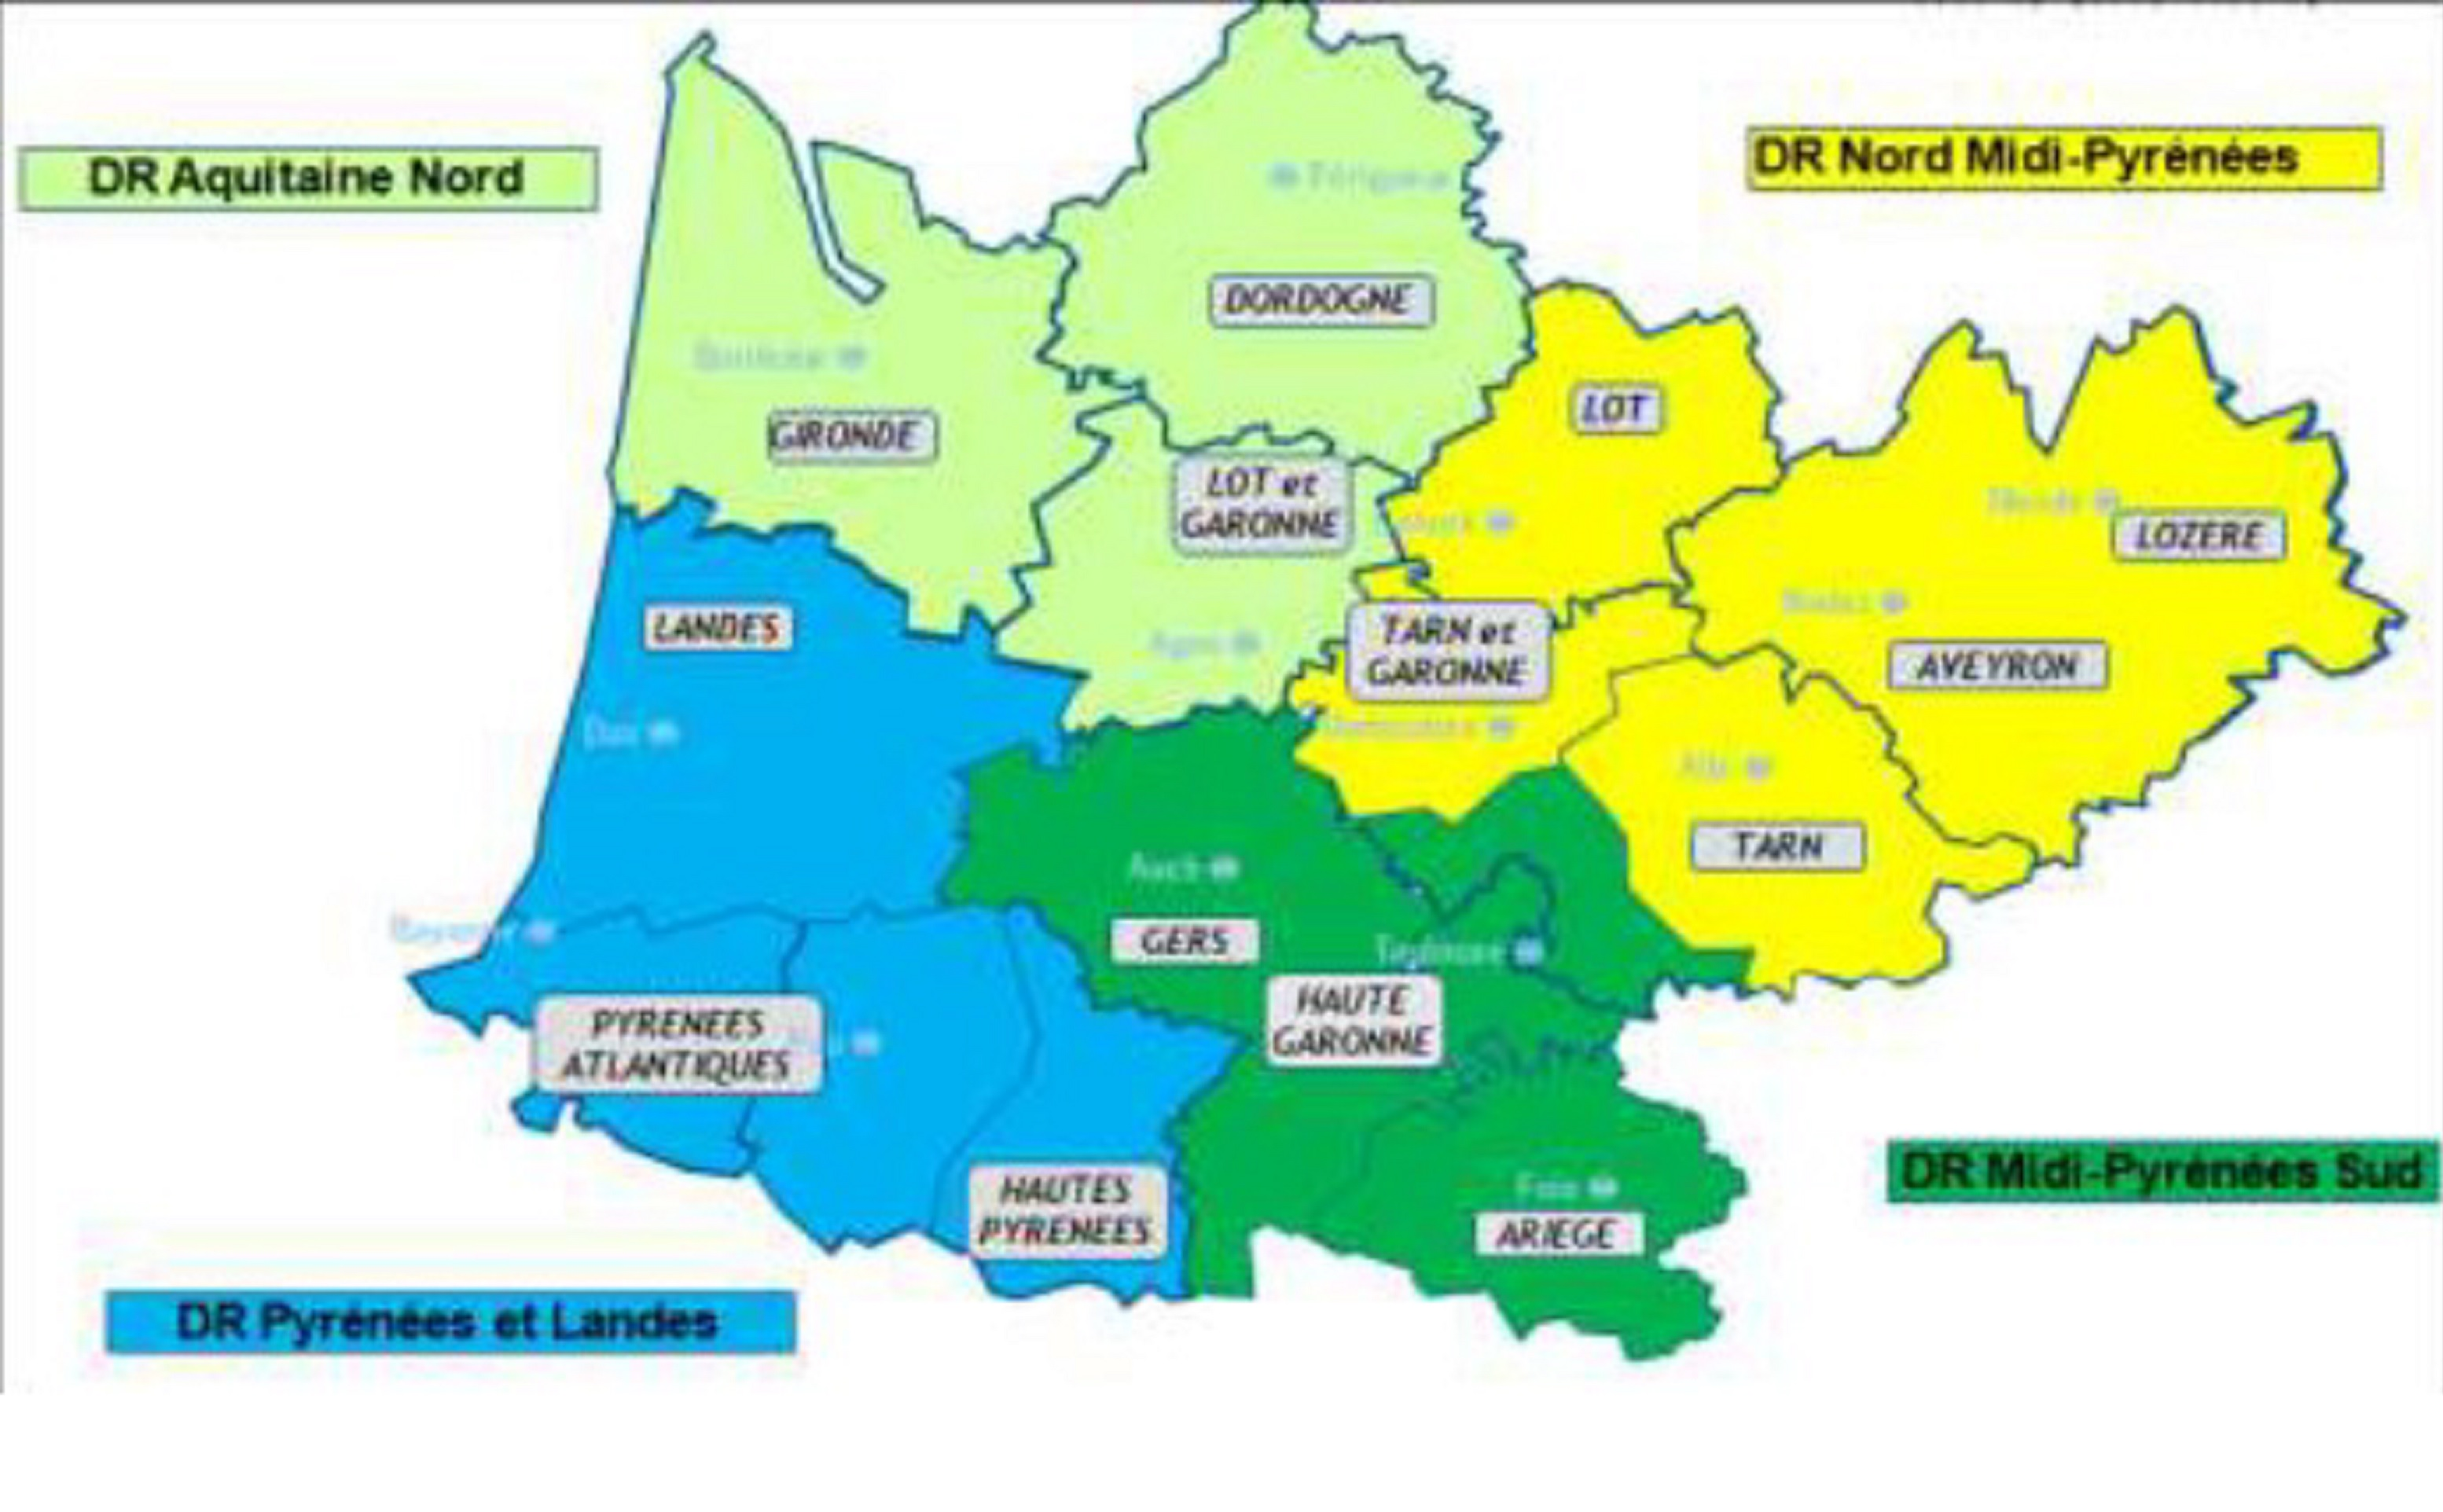
\includegraphics[width=13cm]{dir.jpg}
\caption{\label{dirso}la répartition des 4 DR à la maille Sud Ouest}
\end{figure}
Le rôle des DR est de construire un projet stratégique de région, d'être responsable de la vie des concessions et de la conduite des opérations et de piloter sa performance financière, sociale, technique et patrimoniale.

\subsection*{Direction Technique}
 Elle a été créée pour répondre aux enjeux d'ERDF en inter-région Sud Ouest et pour s'adapter aux évolutions de l'environnement externe et interne.
Elle a aussi un enjeu financier à travers les prévisions budgétaires annuelles attribuées pour chaque Direction Régionale.
Cette Direction Technique présidée par Thierry MARTINEZ, a un champ d'action dans toutes les DR et
dispose de 3 sites basés à TOULOUSE (31), BORDEAUX (33) et AGEN (47).
Son rôle est de préparer et porter les politiques techniques, d'animer les 3 domaines métiers en inter-région (patrimoine – réseau – Poste Source), d'assurer les études électriques en co-construction avec les DR.
Pour exercer ses différentes missions, la Direction Technique est organisée en 7 pôles d'activités
qui sont:
\begin{itemize}
\item Pôle Études et Maîtrise Ouvrage HTA
\item Pôle Maîtrise Ouvrage Postes Sources
\item Pôle Grand Producteur\footnote{Pendant mon stage de l'année dernière (2013-2014), j'ai développé un outil de suivi et de pilotage d'activité pour ce pôle}
\item Expertise Technique et SI
\item Économie Concessionnaire
\item Politique Industrielle
\item Politique Programme Performance
\end{itemize}
Je me situe quant à moi dans le \og Pôle Études et Maîtrise Ouvrage HTA\fg{} que je vais vous présenter.\\ Le pôle \og Études et Maîtrise d'ouvrage HTA\fg{} est constitué de 3 métiers, comme le montre le schéma~\ref{metier} ci-dessous:
\begin{figure}[h]
\centering
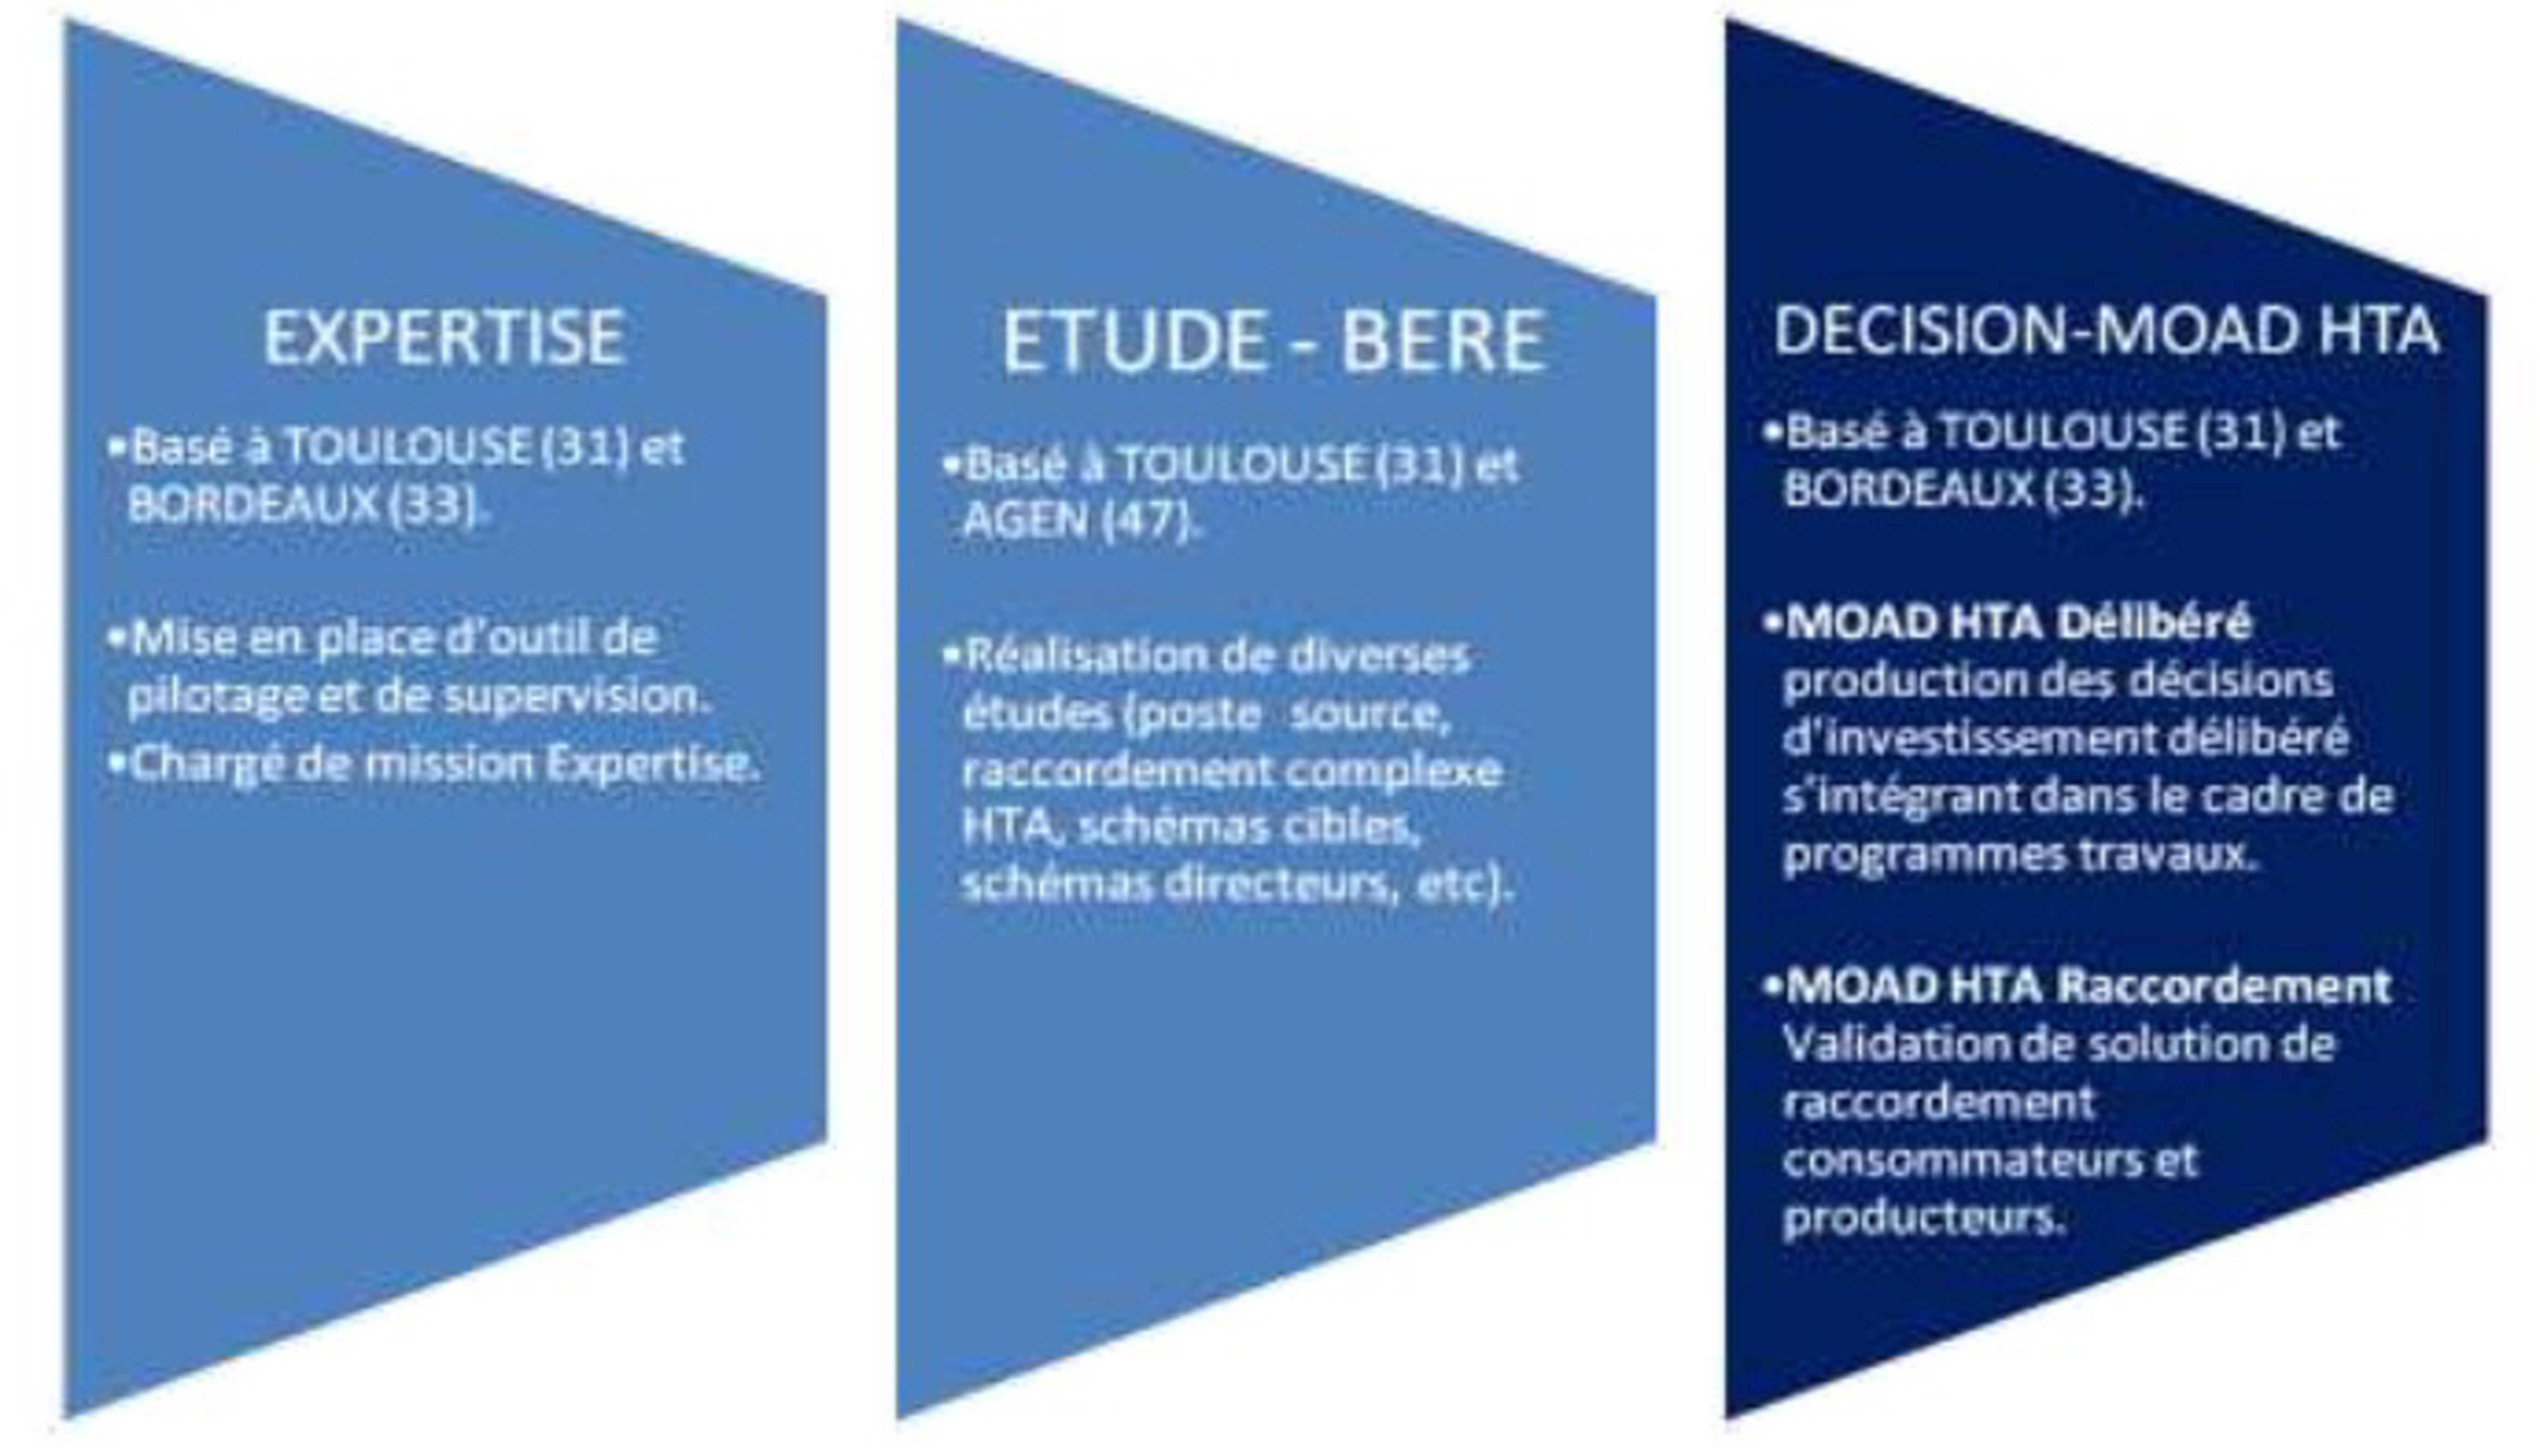
\includegraphics[width=13cm]{metier.jpg}
\caption{\label{metier}les métiers du pôle \og Études et Maîtrise d’ouvrage HTA\fg{}}
\end{figure}
Le but de ma mission est donc de créer un portail de travail collaboratif afin que les BERE ainsi que la maitrise d'ouvrage pour qu'il puisse travailler ensemble afin d'améliorer leurs résultats. 

\chapter{Présentation du projet} % Main chapter title

\label{Chapter2} % Change X to a consecutive number; for referencing this chapter elsewhere, use \ref{ChapterX}

\lhead{Chapitre 2. \emph{Présentation du projet}} % Change X to a consecutive number; this is for the header on each page - perhaps a shortened title
\section{Contexte}
L'environnement à ERDF est varié, suivant l'adage à chaque usage son outil.
Résultats : un environnement vaste d'outils qui ne dialoguent pas toujours entre eux, dont leur
emplacement de stockage n'est trop souvent connu que de quelques initiés, dont on ignore les
différentes versions utilisées et par qui, et enfin des outils qui, au lieu de répondre à la totalité des
besoins, en sollicitent d'autres.
Face aux enjeux de Qualité et de Performance sans cesse grandissant, une nécessaire mise à plat de
l'ensemble des outils et un indispensable espace commun de partage, conduisent à imaginer la
création d'un espace commun y permettant d'y répondre.
La mise en réseau d'un espace de partage commun doit à la fois favoriser les échanges entre entité
mais aussi assurer l'unicité des versions des outils utilisés sur l'ensemble de la Direction
Inter-régionale Sud-Ouest.
\section{Objectif}
L'outil à développer devait répondre aux exigences suivantes:
\begin{enumerate}
\item Un accès rapide à une information pertinente
\begin{itemize}
\item Fournir un accès rapide (il s'agit là d'organiser l'accès à l'information en en limitant le
nombre de gestes nécessaires) à une information ciblée, pertinente et mise à jour systématique.
\item Optimiser la recherche d'information par le biais d'un moteur de recherche performant.
\end{itemize}
\item Un meilleur partage des connaissances et des expériences
\begin{itemize}
\item Favoriser le travail collaboratif et l'échange
\item Capitaliser et partager les savoirs et les connaissances (référentiels communs …)
\item Favoriser la mise à disposition d'applications et d'outils informatiques en limitant un accès
unique suivant la règle « une application un seul accès ».
\end{itemize}
\item Des contenus pouvant devenir de plus en plus hétérogènes\\
Le portail doit être conçu de manière à pouvoir accepter des contenus dont on ignore à ce jour la
forme et par conséquent il doit permettre de:
\begin{itemize}
\item Diffuser et/ou recevoir des informations ascendantes, descendantes et transversales de
communication interne et propres au réseau d'acteurs concernés.
\item Sous différentes formes : courriel, flux RSS, document à télécharger, liens hypertexte, flux de
travail
\item Tout utilisateur, disposant de droits spécifiques à la mise à jour du portail, doit pouvoir, sans
connaissance particulière du langage utilisé, de manière intuitive mettre en ligne des liens, des
documents, des outils.
\end{itemize}
\item Une réponse aux contraintes du réseau d'acteurs
\begin{itemize}
\item Améliorer la circulation, l'historisation et le partage d'informations entre les acteurs internes
\item Favoriser la communication et les échanges entre les structures sur l'ensemble du réseau
d'acteurs en allégeant la communication par courriel
\item Favoriser l'unicité d'outils communs
\item Garantir la qualité des données (et identifier celles susceptibles d'être erronées).
\end{itemize}
\item Accessible depuis un smartphone ou une tablette.
\end{enumerate}
\section{Outils techniques}
Pour atteindre l'objectif décrit, j'avais à ma disposition: 
\begin{itemize}
\item Deux serveurs web apache. Un serveur était dédié à l'environnement de développement et l'autre à l'environnement de production.
\item l'annuaire LDAP pour gérer l'authentification
\item deux certificats de sécurités pour les serveurs 
\item un gestionnaire de contenu qui sera défini dans la partie \og phase d'étude\fg{}
\item netbeans comme environnement de développement intégré
\end{itemize}  
\section{Étude de l'existant}
L'outil existant était juste un gestionnaire Lotus Notes\footnote{Lotus Notes est un logiciel de travail collaboratif développer par IBM. Il est beaucoup utiliser dans les entreprises pour la gestion des projets, les courriels et les échanges d'informations}. Cet outil ne répondait pas parfaitement à leurs besoins car son système de gestionnaire de fichier n'était pas efficace tout en sachant que la bonne gestion des fichiers pour eux était très importante. De plus il n'offrait pas toutes les fonctionnalités souhaitées par l'entreprise.
On a donc décidé de développer un portail collaboratif capable de résoudre le manque que présentait Lotus Notestout en rajoutant de nouvelles fonctionnalités. 
\chapter{Présentation du travail réalisé} % Main chapter title

\label{Chapter3} % Change X to a consecutive number; for referencing this chapter elsewhere, use \ref{ChapterX}

\lhead{Chapitre 3. \emph{Présentation du travail réalisé}} % Change X to a consecutive number; this is for the header on each page - perhaps a shortened title
\section{Phase d'études}
Vu les raisons mentionnées dans la partie étude de l'existant, la fonctionnalité la plus importante dans ce projet était la gestion documentaire. Il existe de nombreuses solutions répondant à ce besoin, comme \textit{SharePoint de Microsoft}, \textit{FileNet d'IBM}, etc... La plupart de ces solutions sont payantes et souvent ne répondent pas à 100\% aux besoins des entreprises. Alors il existe des solutions alternatives open source: les gestionnaires de contenus appelés CMS (\textit{Content Management System}). L'open source gagne chaque année de nouveaux domaines d'applications. Les solutions proposées sont de plus en plus matures, et sont de vraies alternatives aux solutions historiques, propriétaires\cite{ged}. Pour faire le choix, j'ai procédé à une étude des solutions existantes.
\subsection{Étude des solutions}
De nos jours ils existent plusieurs gestionnaires de contenu. Les solutions proposées par ces derniers sont différentes les unes des autres.
Afin de bien choisir mon CMS, j'ai essayé de répondre aux questions publiées dans le livre\cite{Choisir}  \textit{200 questions pour choisir un CMS} de Smile\footnote{Smile est le premier intégrateur français et européen de solutions open source.}. Pendant leur passage à l'université Paris Ouest Nanterre La Défense pour un séminaire sur l'open source, ils nous ont beaucoup parler des CMS du marché ainsi que des livres blancs téléchargeables sur leur site web. 
Les questions\footnote{toutes les questions viennent du livre Smile\cite{choixPage}} auxquelles j'ai répondu et qui étaient intéressantes pour ce projet sont indiquées dans le tableau~\ref{questionsChoix}.\\

\begin{table}[h]
\centering
\begin{tabular}{|p{10cm}|m{2cm}|}
\hline questions & réponses \tabularnewline
\hline est-il possible de définir des types de contenus nouveaux, correspondant à un besoin spécifique & oui \tabularnewline
\hline est-il possible de modifier un type de contenu alors qu'il existe déjà de contenus de ce type & oui \tabularnewline
\hline est-il possible d'ajouter des méta-données & oui \tabularnewline
\hline est-il possible de définir l'arborescence du site, sans limitation de profondeur & oui \tabularnewline
\hline est-il possible de placer un même contenu dans plusieurs pages distinctes ? ceci sans le dupliquer & oui \tabularnewline
\hline est-il possible de gérer plusieurs sites au sein d'un unique back-office & oui \tabularnewline

\hline existe-t-il une médiathèque & oui \tabularnewline
\hline existe-t-il des fonctions de traitement d'images intégrées & oui \tabularnewline
\hline l'interface de contribution est-elle facile à prendre en main pour les non initiés & oui \tabularnewline
\hline est-il possible de définir des habilitations de validation distinctes selon les rubriques & oui \tabularnewline
\hline le valideur peut-il avoir un aperçu du contenu dans la page où il sera publié et avec le gabarit correspondant & oui \tabularnewline
\hline le CMS permet-il de produire des publications autres que Html\footnote{Hypertext Markup Langage est le format de données conçu pour représenter les pages web} ? par exemple pour les mobiles, pour les tablettes, etc. & oui \tabularnewline
\hline est-il possible de diffuser des contenus sous la forme de flux RSS\footnote{ces flux représente un moyen simple d'être tenu informé des nouveaux contenu d'un site web, sans avoir à le consulter\cite{ccm}} & oui \tabularnewline
\hline peut-on rendre certaines parties du site privatives pour des groupes ou utilisateurs & oui \tabularnewline
\hline les habilitations peuvent-elles être définies par groupes d'utilisateurs & oui \tabularnewline
\hline est-il possible de définir précisément les droits sur chacune des actions élémentaire de back-office & oui \tabularnewline
\hline le CMS possède-t-il une fonction de recherche intégrée & oui \tabularnewline
\hline peut-on gérer les utilisateurs depuis un annuaire LDAP\footnote{Protocole d'annuaire sur TCP/IP. Il permet de partager des bases d'informations sur le réseau interne ou externe\cite{ldap}} & oui \tabularnewline
\hline le produit est-il diffusé sous licence open source, ou bien sous une licence commerciale & open source \tabularnewline
\hline workflow pour notifier les utilisateurs & oui \tabularnewline
\hline
\end{tabular}

\caption{\label{questionsChoix}Questions pour choisir un CMS}
\end{table}
\clearpage


\subsection{Solution retenue}
Après avoir répondu à toutes les questions~\ref{questionsChoix}, j'ai regardé la comparaison effectuée par Smile dans le cadre de la présentation des différents CMS du marché\cite{comparaison}. La figure représente le résultat de cette comparaison.
\begin{figure}[h]
\centering
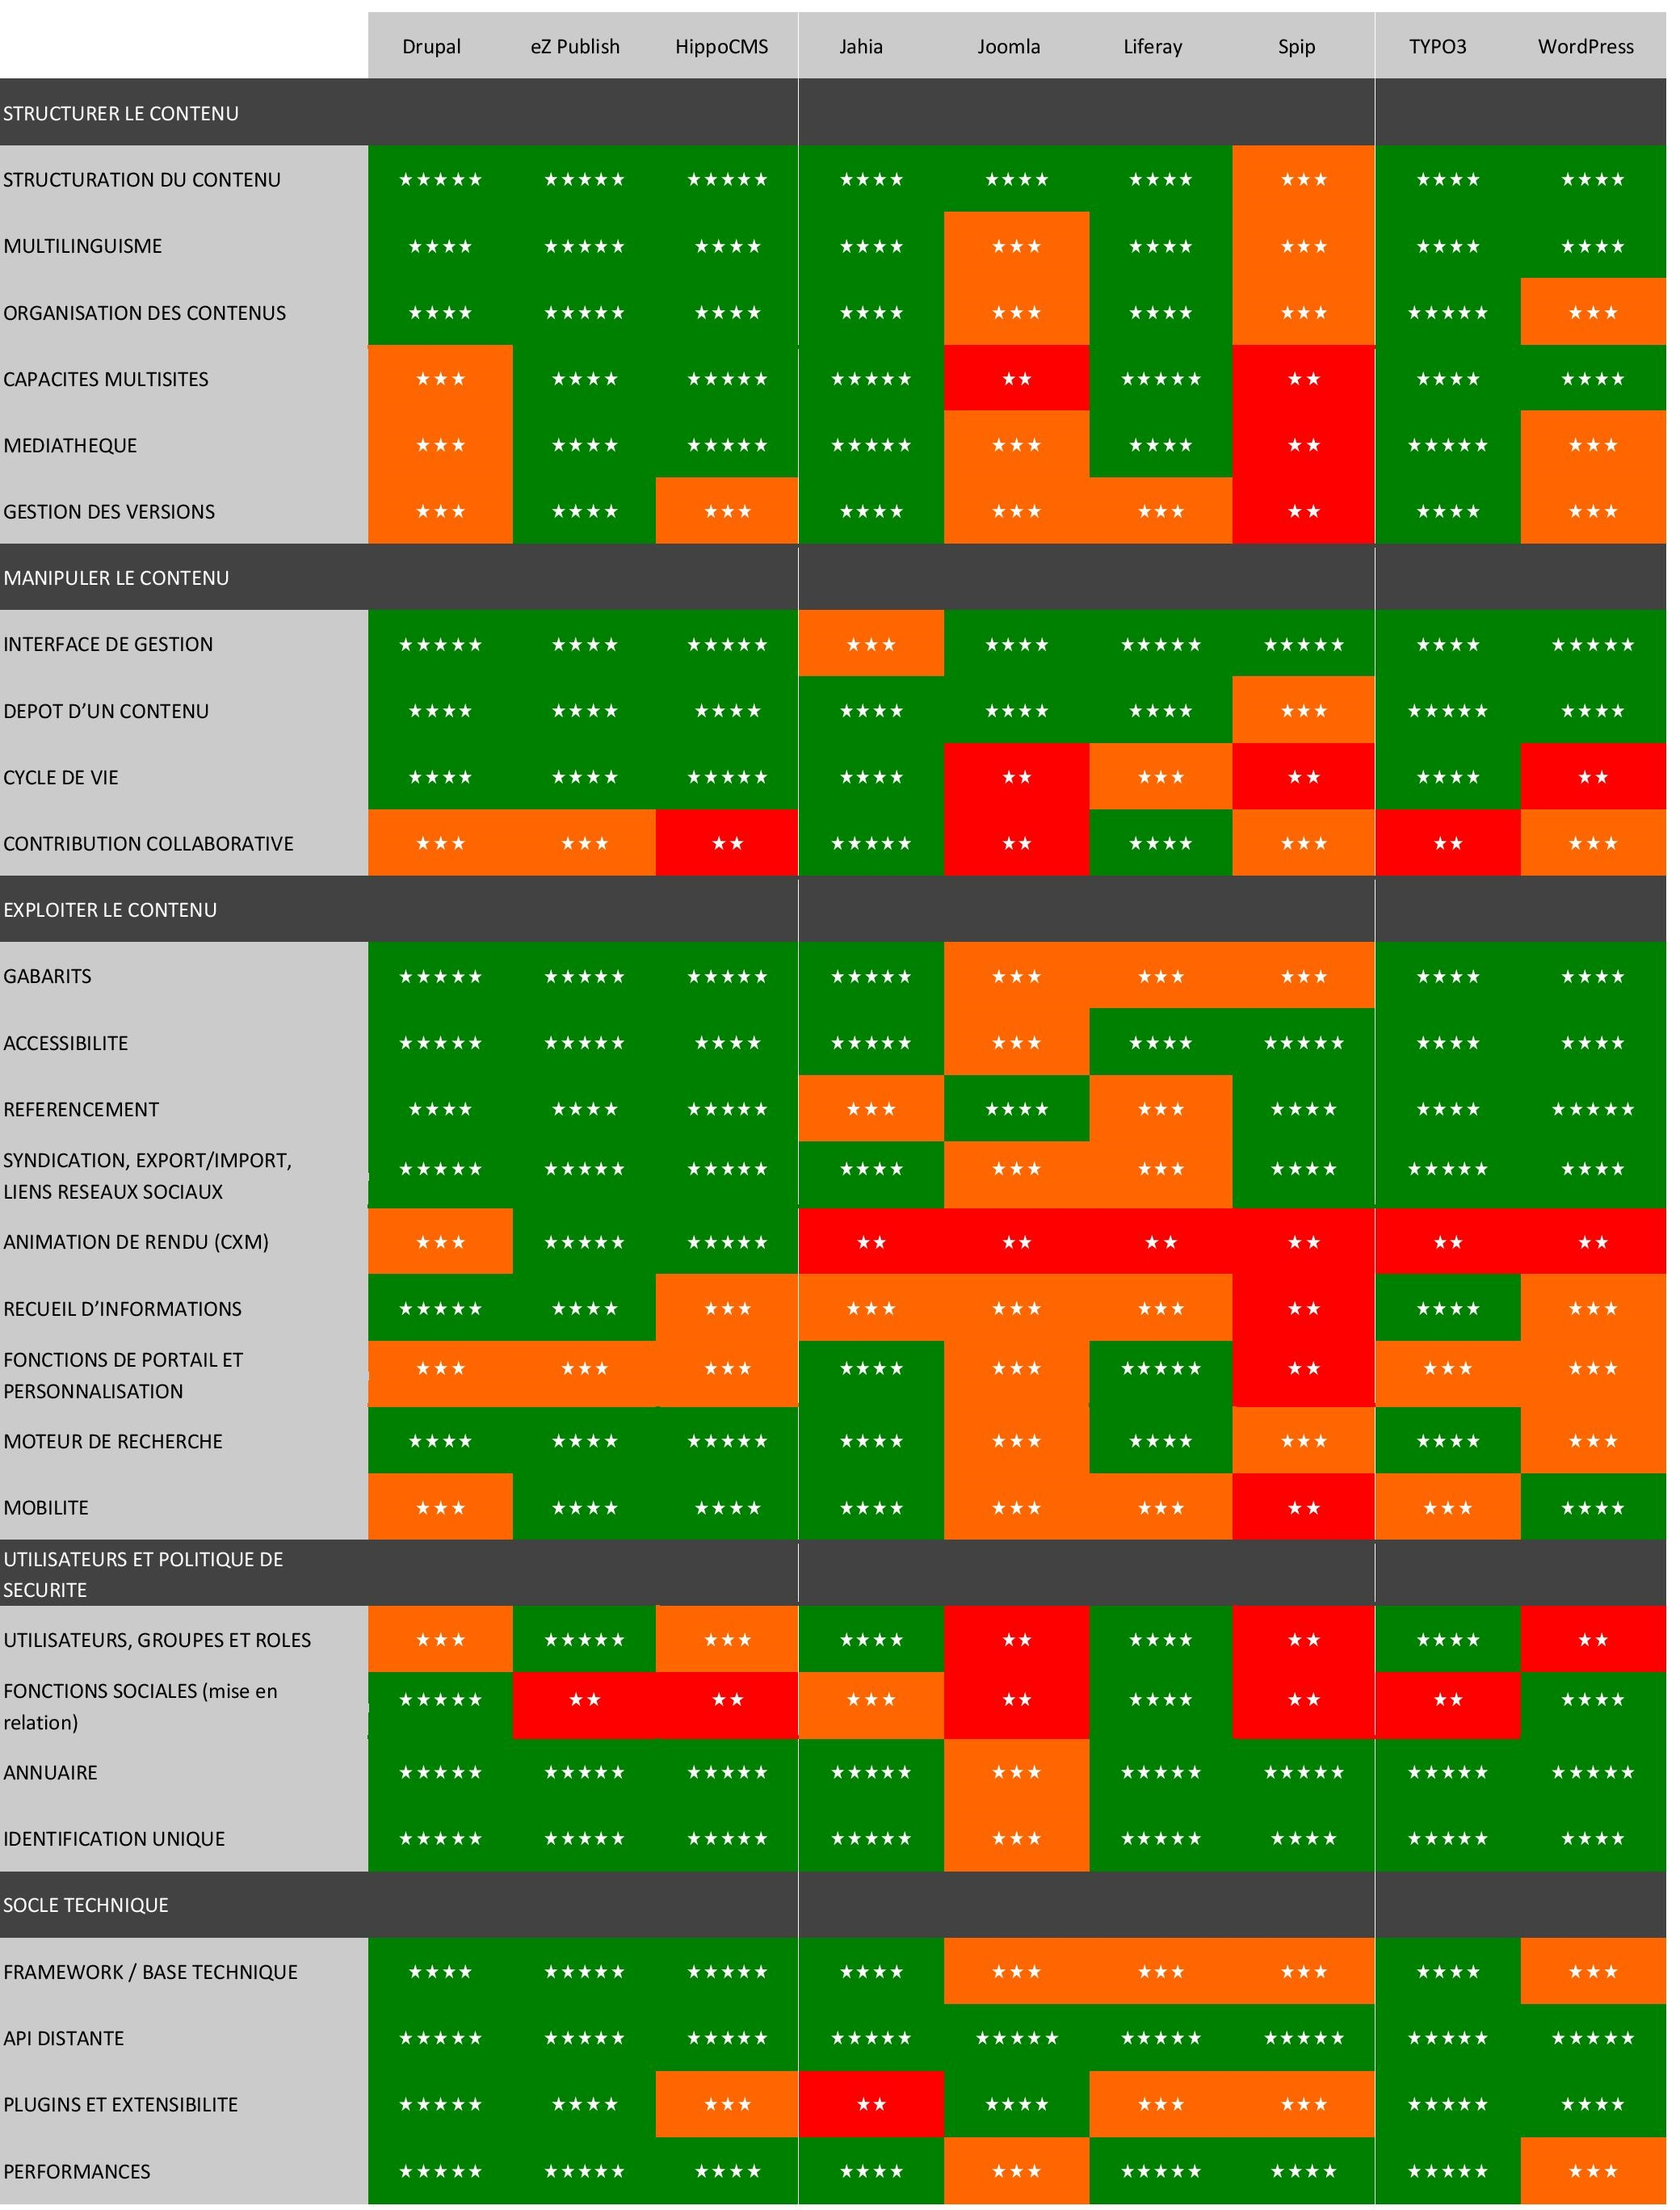
\includegraphics[width=14.5cm]{comparaison.jpg}
\caption{\label{comparaisonRef}Comparaison entre les CMS\cite{comparaison}}
\end{figure}
\clearpage
Après cette comparaison nous remarquons que les CMS qui se détachent des autres sont:
\begin{itemize}
\item Typo3: qui est un très bon gestionnaire de contenu mais il n'a pas été retenu parce qu'il est moins performant sur les \og Portails Intranet\fg{}\cite{typo3} et aussi il ne nous permettait pas d'organiser notre portail sous forme d'espace.
\item Jahia: a un très beau score dans le tableau de comparaison, mais ce CMS n'a pas été retenu parce qu'il ne permettait pas d'organiser notre portail sous forme d'espace.
\item Ez publish: obtient lui également un beau score dans la comparaison, en revanche il n'est pas assez documenter.
\item Drupal: même s'il reste un peu en retrait sur la mise en place d'une architecture multi-sites, drupal a été la solution que nous avons choisi car il est très bien documenté, il y a une forte communauté derrière pour assurer le bon fonctionnement de ce CMS et aussi propose plusieurs modules dont \og open atrium\fg{} qui répondent parfaitement à nos besoins. \\Sans me le dire lors de ma phase d'étude pour le choix du CMS, mon tuteur en entreprise avait également fait des recherches par rapport au type de CMS que je pouvais utiliser et c'est Drupal qu'il avait choisi.
\end{itemize}
\section{Développement}
La phase de développement fut l'une des phases les plus importantes dans ce projet, car elle sert à mettre en place l'outil demandé grâce aux différentes solutions qui ont été retenues.\\
Durant le développement, plusieurs réunions avec les futurs utilisateurs ont été organisée car on travaillait en méthode agile, donc à la fin de chaque une itération, les utilisateurs devaient tester la ou les fonctionnalités développées puis les valider si elle(s) répond(ent) à leur besoins.\\
Dans cette partie nous allons parler des fonctionnalités qui ont pu être réalisées et également celles qui n'ont pas pu l'être.
\subsection*{Tâches réalisées}
Avant de commencer à réaliser le développement, nous avons effectué quelques réunions avec les super utilisateurs\footnote{les super utilisateurs sont les personnes représentants les différents profils (BERE, MOAD) }. 
Le but de ces réunions était de pouvoir comprendre ce que les clients voulaient et de s'assurer qu'on a bien compris ce qu'ils voulaient. Au bout de 3 réunions, nous avons dressé une nouvelle liste de fonctionnalités avec des priorités différentes. Ces fonctionnalités n'étaient pas définitives, car elles pouvaient être modifiées par rapport à la faisabilité ou au besoin.
La nouvelle liste de fonctions à réaliser était: 
\begin{itemize}
\item l'authentification via l'annuaire \textbf{\textit{GARDIAN SESAME}}: tout accès au portail devait passer par l'annuaire gardian sesame afin de sécuriser le site. Cette tâche avait une priorité élevée car tous leurs outils utilisaient ce système d'authentification, donc il n'était pas question de réaliser un autre outil avec un autre système d'authentification.\\
Pour accomplir cette tâche j'avais chercher des modules drupal permettant de gérer les connexions LDAP, mais les modules trouvés ne prenait pas en compte le type d'authentification que je devais réalisé. Alors pour résoudre ce problème j'ai dû aller dans le cœur de drupal pour modifier le système de connexion.
\begin{lstlisting}
	<?php
	// inclusion des classes necessaires
	// pour l'authententification LDAP 
	include("ldap/LdapAuth.php");
	$options= array(
	// liste des serveurs LDAP sur lesquels on doit tenter 
	//la connexion pour authentification. 
	//L'ordre est important.
	'servers' => array("lien-annuaire-1","lien-annuaire-2"),
	'use_ldaps'=> true,
	'bind_dn'=> "uid=identApp,ou=ou-1,dc=mydc",
	'bind_pwd'=> 'XXXXXXX',
	// base de recherche dans l'annuaire 
	//pour la recherche d'utilisateur
	'searchBase'=> "ou=ou-2,dc=mydc",
	// fermeture automatique de la 
	//connection LDAP a la fin de 
	//l'authentification (utile si 
	//plusieurs authentification dans le script)
	'closeConnection'	=> true,
	// delai maximum de recherche LDAP (pour la recherche 
	//de l'utilisateur pour recuperation du DN)
	'timelimit'=> 1
	);
	$ldapAuth=new LdapAuth($options);
	
	try {
		$nni = $form_state['values']['name'];
		$pass = $password;
		$date = date('Y-m-d H:i:s');
		$ldapbind=$ldapAuth->authenticateUser($nni, $pass);
		
	} catch (LdapException $e) {
	 
		$resultat=$e->getMessage();
	}
\end{lstlisting}
\item les espaces: dans le portail, on avait plusieurs profil (moad, bere, public, hypervision, commun) et rôle; donc chaque profil avait son propre espace de travail.
\item la gestion des droits: on avait différents rôles et groupes de travail dans chaque espace, donc on devait pouvoir gérer les droits des utilisateurs en fonctions des groupes qu'ils appartiennent ou des rôles qu'ils possèdent selon l'espace dans lequel ils se trouvent. Cette fonctionnalité avait également une priorité élevée  
\item trombinoscope: avec une priorité moyenne, cette fonctionnalité permet aux utilisateurs de retrouver facilement les contacts des autres utilisateurs. Comme drupal fonctionne avec des modules, nous avons mis en place un module permettant de récupérer les informations (nom, prénom, mail, photo, téléphone) des utilisateurs et de les afficher selon la demande de l'utilisateur.
\item gestion documentaire: elle était la partie la plus importante du projet, les utilisateurs devaient pouvoir partager leurs documents dans leur espace tout en gérant également les droits de lecture et d'écriture sur ces documents avec des systèmes de notification selon qu'on soit abonné ou pas. Alors pour cette fonctionnalité, on avait opté pour une première solution qui consiste à utiliser filedepot\footnote{filedepot est un module de gestionnaire de fichier sous drupal}. Après avoir mise en place cette solution, les clients l'ont jugé un peu compliquée, alors nous avons développé une autre solution plus simple que la première tout en gardant la première solution au cas où on voudra revenir la dessus car cette dernière présente de nombreuses fonctionnalités intéressantes.
\item gestion de types de contenus: l'administrateur devait pouvoir créer différents types de contenus comme par exemple un article avec des photos, des liens vers d'autres documents etc... De natif, drupal gère la gestion des types de contenus, donc la mise en place de cette solution n'a pas été compliquée
\item forum: le forum permet aux utilisateurs de pouvoir échanger par rapport à un sujet. Cette fonctionnalité avait une priorité faible. 
\item foires aux questions: comme pour le forum, cette fonctionnalité avait également une priorité faible. Elle a été réalisée grâce à un module FAQ de drupal.
\item gestion des réservations: avant, les utilisateurs utilisaient un fichier excel pour réservation des voitures, des salles de conférences, des bureaux etc. Alors on a intégré dans notre outil un système de réservation plus simple et plus fiable. Cette fonctionnalité avait une priorité élevée.
\item tableau de bord: ce tableau permettait à l'hyperviseur de voir les statistiques sous forme de graphes, camembert etc. Elle avait une priorité élevée.
\item carte: avec une priorité élevée, on devait afficher sur la carte les différents postes sources avec leurs informations (liens vers les études correspondantes aux postes sources, le nombre de clients etc...)
\item formulaire de demande: ce formulaire de demande servait en quelque sorte comme un outil de suivi de projet ou de tâches. Les utilisateurs peuvent s'adresser entre eux, des demandes de tâches et en même temps suivre l'état d'avancement des tâches demandées. cette fonctionnalité avait une faible priorité.
\end{itemize}
\subsection*{Tâches non réalisées}\label{nonrealise}
Parmi les fonctionnalités citées ci-dessus, la plupart a été réalisée sauf deux qui sont: 
\begin{itemize}
\item tableau de bord: le tableau de bord n'a pas pu être réalisée car c'est mon tuteur en entreprise qui devait me fournir la liste des données ainsi que les types de calculs qu'on devait faire pour les statistiques. Malheureusement vers la fin du mois de juillet, il est tombé malade et il n'est retourné qu'au mois de septembre. En son absence, on a chargé une autre personne de s'occuper du suivi de projet mais ce dernière était également en congé et elle n'est retournée que vers mi-août. Alors cette personne n'étant pas au courant de la réalisation du tableau de bord, elle ne pouvait pas m'aider car elle n'avait pas connaissance des données qu'on devait récupérer pour faire les statistiques.\\
On a fait quand même un exemple de tableau de bord avec des données statiques pour montrer que c'était faisable.
\item carte: pour les mêmes raisons que le tableau de bord, l'absence de mon tuteur à mis en suspension la réalisation de cette fonctionnalité car c'est lui qui devait me fournir le reste des éléments pour faire la carte. On avait déjà commencé à réaliser cette fonctionnalité, une grande partie ayant été faite, ils (les utilisateurs) pourront eux même continuer avec le reste car il n'y a plus de code à faire mais juste la saisie des données.
\end{itemize}

\chapter{Conclusion} % Main chapter title

\label{Chapitre4} % For referencing the chapter elsewhere, use \ref{Chapter1} 

\lhead{Chapitre 4. \emph{Conclusion}} % This is for the header on each page - perhaps a shortened title
Dans ce travail de recherche, nous avons étudier les variations par rapport aux prévisions dans la gestion des projets informatiques. Nous avions pour objectif d'étudier les variations et de proposer un modèle de gestion de ces variations pendant la gestion du projet.\\
Nous avons proposer deux solutions: une première solution basée sur les PSEE et une seconde solution avec un fichier excel.\\
La première solution est composée de trois parties: le méta-modèle pour décrire les procédés, la technique de détection des variations et le plan de correction pour la variation détectée.\\
La seconde solution a été mise en place suite à une discussion avec un chef de projet chez Alstom. C'est un macro excel permettant de détecter les variations grâce aux paramètres qu'on lui fournit et nous affiche les résultats sous forme de graphe. \\
Même si ces solutions permettent de détecter quelques variations, et aident le chef de projet dans la prise de décision; elles ne peuvent pas détecter tous les types de variations.\\
\textbf{Limites et perspectives}: les limites et les perspectives d'amélioration de nos deux solutions sont:\\
\textbf{Solution 1}:\\
Notre première solution est assez limité car elle ne permet pas d'anticiper la détection des variations. La variation n'est détectée que lorsque les tâches sont terminées.\\
\textbf{Solution 2}:\\
Les diagrammes résultant de l'exploitation de notre modèle de fichier Excel initialement mis en place et nous permettent à travers des représentations graphiques de voir systématiquement la variation sur les dates de début et de réalisation des tâches. \\
Par rapport aux diagrammes~\ref{graphe1} et~\ref{graphe2} on pourra améliorer ces derniers en traçant une droite horizontale qui représente la date de validité (date à laquelle les données ont été mises à jour), on aurait pu séparer les taches précédentes des tâches futures à venir~\ref{graphe4}.
\begin{figure}[h]
\centering
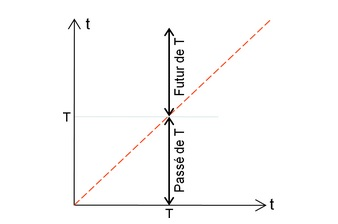
\includegraphics[width=9cm]{graphe4.jpg}
\caption{\label{graphe2}Amélioration}
\end{figure}
D'autres types d'indicateurs peuvent également être mis en  place en fonction des besoins. On pourra par exemple mettre en place un tableau de synthèse de variations qui pourra être importé dans un autre outil etc.



%----------------------------------------------------------------------------------------
%	BIBLIOGRAPHY
%----------------------------------------------------------------------------------------

\label{Bibliographie}

\lhead{\emph{Bibliographie}} % Change the page header to say "Bibliography"

\bibliographystyle{unsrtnat} % Use the "unsrtnat" BibTeX style for formatting the Bibliography

\bibliography{Bibliography} % The references (bibliography) information are stored in the file named "Bibliography.bib"

\end{document}  